\subsection[Projekt interfejsu użytkownika]{Projekt interfejsu użytkownika}

\begin{figure}[H]
    \centering
    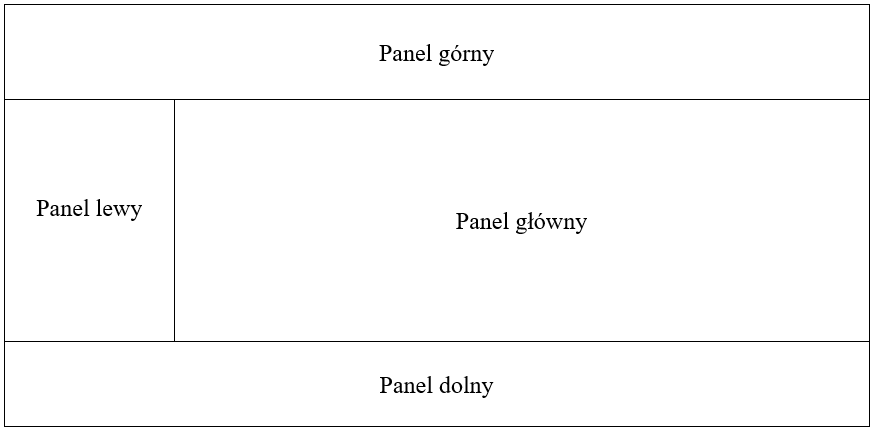
\includegraphics[width=\textwidth]{gui}
    \caption{Schemat układu strony}
    \label{fig:gui}
\end{figure}

\begin{table}[H]
    \begin{tabular}{|p{2cm}|p{12cm}|}
        \hline
        \textbf{} & \textbf{Panel górny} \\
        \hline
        Opis: & Panel górny odpowiedzialny jest za uświadamiania zawartości strony.
        Znajduje się tam logo z nazwą systemu. \\
        \hline
        Komponenty: & Logo \\
        \hline
    \end{tabular}  
    \label{tab:gui1}
\end{table}

\begin{table}[H]
    \begin{tabular}{|p{2cm}|p{12cm}|}
        \hline
        \textbf{} & \textbf{Panel lewy} \\
        \hline
        Opis: & Panel lewy zawiera etykiety informujące o zawartości
        panelu głównego i dolnego. \\
        \hline
        Komponenty: & Etykieta informująca o obecności formularza\newline
         Etykieta  informująca o obecności
          listy aktywnych urządzeń wykonujących\newline
         Etykieta informująca o obecności wiadomości 
         otrzymanych od urządzeń wykonujących \\
        \hline
    \end{tabular}  
    \label{tab:gui1}
\end{table}

\begin{table}[H]
    \begin{tabular}{|p{2cm}|p{12cm}|}
        \hline
        \textbf{} & \textbf{Panel główny} \\
        \hline
        Opis: & Panel główny udostępnia kontrolki odpowiedzialne za 
        wysłanie rządania do urządzenia wykonującego. \\
        \hline
        Komponenty: & Pole tekstowe na treść żądania \newline
         Kontrolki do wyboru parametrów testu\newline 
         Przycisk do wysłania żądania\newline
         Przycisk do załadowania odpowiedzi \newline
        otrzymanych od urządzenia wykonującego \\
        \hline
    \end{tabular}  
    \label{tab:gui1}
\end{table}

\begin{table}[H]
    \begin{tabular}{|p{2cm}|p{12cm}|}
        \hline
        \textbf{} & \textbf{Panel dolny} \\
        \hline
        Opis: & Panel dolny prezentuje wiadomości otrzymane od 
        urządzeń wykonujących takie jak raporty i informacje o
         błędach. \\
        \hline
        Komponenty: & Lista wiadomości \\
        \hline
    \end{tabular}  
    \label{tab:gui1}
\end{table}